\documentclass[12pt]{article}

\usepackage{sbc-template}

\usepackage{graphicx,url}

\usepackage[brazil]{babel}   
%\usepackage[latin1]{inputenc}  
\usepackage[utf8]{inputenc}  
% UTF-8 encoding is recommended by ShareLaTex

     
\sloppy

\title{Exercício 4 - Laboratório de Redes de Computadores}

\author{Leonardo G. Carvalho\inst{1}, Matheus S. Redecker\inst{1}}


\address{Pontifícia Universidade Católica do Rio Grande do Sul - PUCRS
  \email{  \{leonardo.gubert\}\{matheus.redecker\} @acad.pucrs.br}
}

\begin{document} 

\maketitle


\section{}
Server 10.32.143.223 \\
Client 10.32.143.194

\section{} 
\subsection{i)}
Com os resultados obtidos montamos um gráfico que está explicitado na figura \ref{1i}. Nele é visto que com a janela muito baixa temos pouco throughput, e a medida que a janela aumenta o throughput também aumenta, até chegar a um ponto que estabiliza, esse ponto está em aproximadamente 94Mbits/s.
\begin{figure}[ht]
\centering
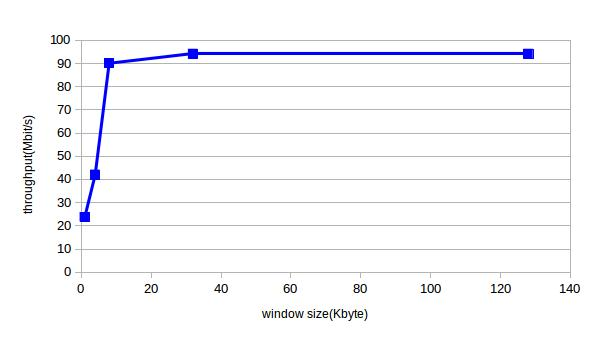
\includegraphics[scale=0.5]{primeiro.jpg}
\caption{}
\label{1i}
\end{figure}

\newpage{}
\subsection{ii)}
Com os resultado obtidos montamos os gráficos para mostrar o throughput representado na figura \ref{1iia} e o jitter representado na figura \ref{1iib}. Como a perda de pacotes foi 0 em todas as transmissões resolvemos não montar um gráfico para essa medida. O jitter é grande quando temos uma taxa de envio baixa, mas a medida que aumentamos ele chega a ficar estável. Já o throughput é igual a taxa de envio.   
\begin{figure}[ht]
\centering
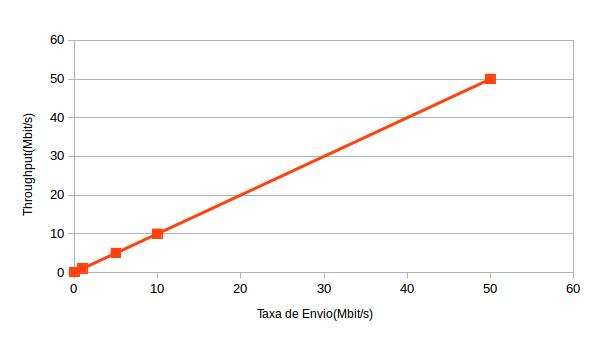
\includegraphics[scale=0.5]{segundothr.jpg}
\caption{}
\label{1iia}
\end{figure}

\begin{figure}[ht]
\centering
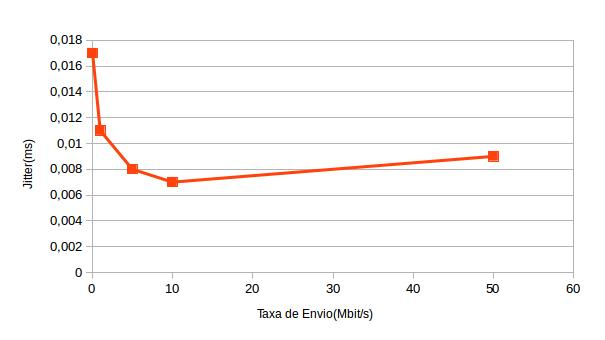
\includegraphics[scale=0.5]{segundojitt.jpg}
\caption{}
\label{1iib}
\end{figure}

\newpage{}
\section{}
\subsection{a)}
tc qdisc add dev eth0 root netem delay 100ms 20ms distribution normal
\subsection{b)}
\subsubsection{i)}
Com os resultados obtidos montamos o gráfico que está apresentado na figura \ref{3}, nele é visto que o throughput aumenta conforme a janela aumenta.

\begin{figure}[ht]
\centering
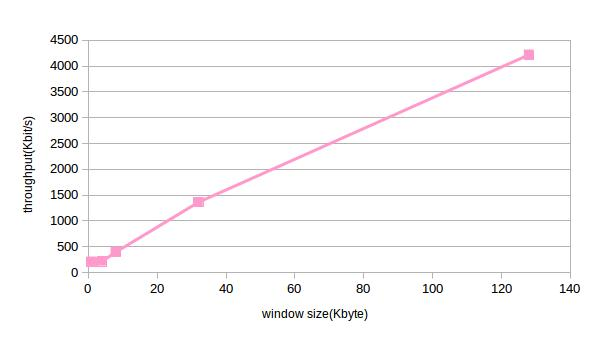
\includegraphics[scale=0.5]{terceiro1.jpg}
\caption{}
\label{3}
\end{figure}
\subsubsection{ii)}
Com os resultado obtidos foi montamos os gráficos para mostrar o throughput representado na figura \ref{3thr}, o jitter representado na figura \ref{3ji} e a perda de pacote representada na figura \ref{3perda}. O throughput aumenta com a taxa de envio e o jitter se mantém na faixa de 20 ms não apresentando algum grande pico. Já a perda de pacotes oscila muito, temos perda de pacote de zero por cento, mas também outras de noventa por cento.

\newpage{} 
\begin{figure}[ht]
\centering
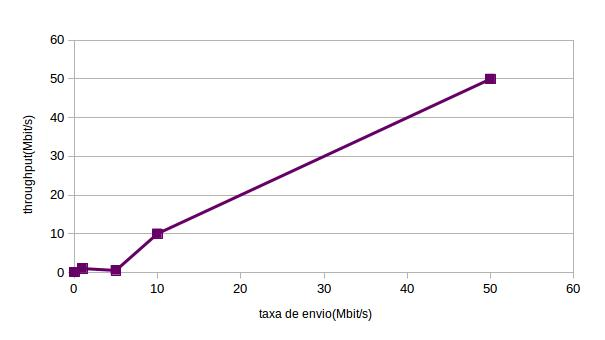
\includegraphics[scale=0.5]{terceirothru.jpg}
\caption{}
\label{3thr}
\end{figure}
\begin{figure}[ht]
\centering
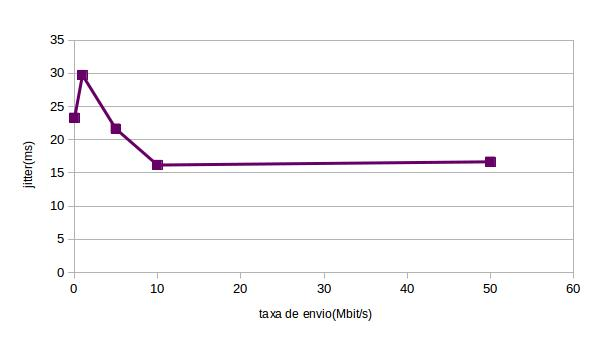
\includegraphics[scale=0.5]{terceirojitt.jpg}
\caption{}
\label{3ji}
\end{figure}
\begin{figure}[ht]
\centering
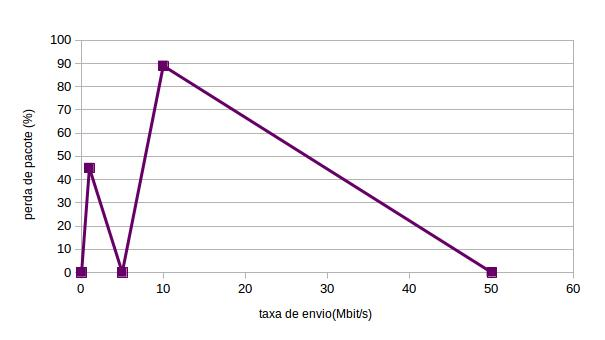
\includegraphics[scale=0.5]{terceiroperda.jpg}
\caption{}
\label{3perda}
\end{figure}
\newpage{} 






\section{}
\subsection{a)}
sudo tc qdisc add dev eth0 root netem loss 5\%
\subsubsection{b)}
\subsubsection{i)}
Com os resultados obtidos montamos o gráfico que está apresentado na figura \ref{4i}. Nele vemos que o throughput estabiliza ao utilizarmos um tamanho de janela grande.

\begin{figure}[ht]
\centering
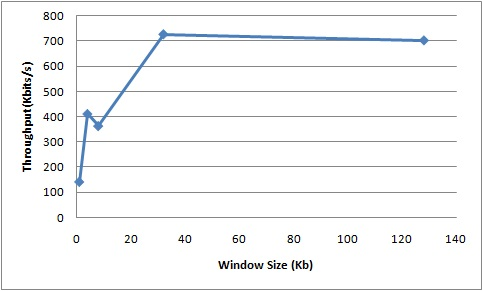
\includegraphics[scale=0.7]{4i.jpg}
\caption{}
\label{4i}
\end{figure}
\newpage{} 

\subsubsection{ii)}
Com os resultado obtidos montamos os gráficos para mostrar o throughput representado na figura \ref{4thr}, o jitter representado na figura \ref{4jit} e a perda de pacotes representado na figura \ref{4perda}. O jitter é grande quando temos uma taxa de envio baixa, mas a medida que aumentamos ele chega a ficar estavél. Já o throughput é igual a taxa de envio.   


\begin{figure}[ht]
\centering
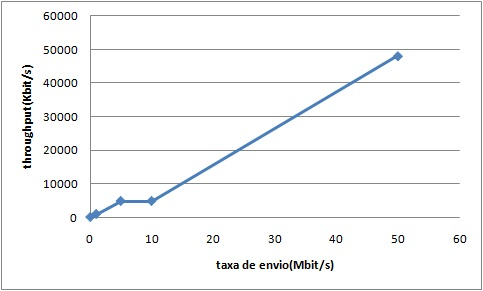
\includegraphics[scale=0.7]{4thr.jpg}
\caption{}
\label{4thr}
\end{figure}

\begin{figure}[ht]
\centering
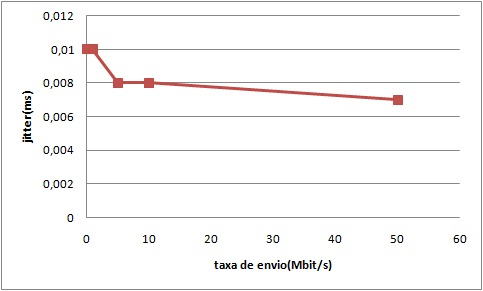
\includegraphics[scale=0.7]{4jit.jpg}
\caption{}
\label{4jit}
\end{figure}

\begin{figure}[ht]
\centering
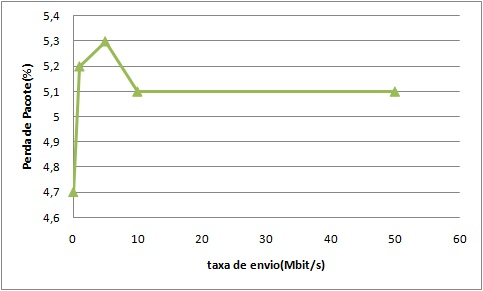
\includegraphics[scale=0.7]{4perda.jpg}
\caption{}
\label{4perda}
\end{figure}




\end{document}
